%% This is a skeleton file to create IEEE style Bibliography list. There is a guide added "create-manual-bib-entry.txt" to manually create popular types of references such as PhD thesis, website, unpublished work etc.
%%
%% Modified by K. Reaz( kahn.reaz@ieee.org)
%% Support sites:
%% http://www.ieee.org/

%%***********************************************************
%% Legal Notice:
%% This code is offered as-is without any warranty either expressed or implied; without even the implied warranty of MERCHANTABILITY or FITNESS FOR A PARTICULAR PURPOSE! 
%% User assumes all risk and can modify as s/he wants.

%%***********************************************************

%package list
\documentclass[conference]{IEEEtran}
\usepackage{cite}
\let\proof\relax
\let\endproof\relax
\usepackage{fullpage,psfrag,amsthm,amsmath,amsfonts,verbatim, mathtools,enumerate,algorithm,algorithmic}
\usepackage{oubraces}
\usepackage{diagbox}
\usepackage{subfig}
\allowdisplaybreaks[2]
\input defs.tex


\begin{document}
%Here goes the title
\title{Tolling for MDP Congestion Games}
\author{authors}
\maketitle
\begin{abstract}
We present a dual perspective on MDP routing games, from a social planner's perspective and individual game player's perspective. In addition, we show that state constraints on MDP  problem can be imposed in an equivalent unconstrained version of the problem with auxiliary rewards. Finally, we apply the formulation on a ride share scenario where the social planner needs to satisfy certain driver density constraints by adjusting local rewards. 
\end{abstract}
%Main body starts
\section{Introduction}
\cite{altman1999constrained}
Although a single population congestion game has been extensively analyzed(CITATION), we adopt the perspective of a global planner to enforce state space constraints without altering individual agent's behaviour. \newline

\textbf{Other's work}: What have others done in this? \newline

In order to enforce global constraints, we treat the routing game as a finite horizion, potential mean-field game that can be solved with a Markov Decision Process(MDP). Using the game reward as planner's control, it can be shown that state constraints can be reformulated as rewards, which in turn motivate game players to achieve a Wardrop Equilibrium that satisfies the constraints. 

In particular, we reformulate state space constraints as a toll or flow based congestion control. Interestingly, it can be shown that a flow based control will not satisfy any state-space constraint by itself. The tolls are then applied to a ride-share scenario where drivers are attempting to maximize individual monetary return.

\section{Notation}\label{notation}
Behcet vs Yoyo vs Einsum
\section{Problem Formulation}\label{problemFormulation}

\subsection{Markov decision processes}
Consider the following linear programming formulation of finite horizon MDP \cite{puterman2014markov}
\begin{equation}
\begin{aligned}
\underset{\substack{y_t\\t\in\mathcal{T}}}{\mbox{min.}} & \sum\limits_{t\in\mathcal{T}}\sum\limits_{s\in\mathcal{S}} \sum\limits_{a\in\mathcal{A}} y_t(s, a)c_t(s, a)\\
\mbox{s.t.} &\sum\limits_{a\in\mathcal{A}} y_{t+1}(s', a) = \sum\limits_{s\in\mathcal{S}}\sum\limits_{a\in\mathcal{A}}\Gamma(s'\mid s, a)y_t(s, a),\\
&\sum\limits_{a\in\mathcal{A}}y_0(s, a)=p_0(s),\\
&y_t(s, a)\geq 0,\quad \forall s, s'\in\mathcal{S}, a\in\mathcal{A}, t\in\mathcal{T}
\end{aligned}\label{MDP}
\end{equation}
where \(\mathcal{S}\) and \(\mathcal{A}\) denote respectively the set of states and actions, \(\mathcal{T}=\{0, \ldots, |\mathcal{T}|\}\) denote the time step, \(y_t(s, a)\) and \(c_t(s, a)\) denote respectively the probability and cost of state-action pair \((s, a)\), \(\Gamma(s'|s, a)\) denotes transition probability from state \(s\) to state \(s'\) given action \(a\), \(p_0(s)\) denotes the probability that the decision processes starts from state \(s\). 
Notice that the initial and dynamics constraints in \eqref{MDP} implies that
\begin{equation*}
\begin{aligned}
\sum\limits_{s\in\mathcal{S}} y_0(s, a)=&\sum\limits_{s\in\mathcal{S}}p_0(s)=1,\\
\sum\limits_{s'\in\mathcal{S}} y_{t+1}(s', a)=&\sum\limits_{s'\in\mathcal{S}}\sum\limits_{s\in\mathcal{S}}\sum\limits_{a\in\mathcal{A}}\Gamma(s'\mid s, a)y_t(s, a)\\
=&\sum\limits_{s\in\mathcal{S}}\sum\limits_{a\in\mathcal{A}}y_t(s, a).
\end{aligned}\label{nomalization}
\end{equation*}
Hence by induction we know that the nomalization constraints on \(y_t(s, a)\) are automatically satisfied for all \(t\in\mathcal{T}\). 

The KKT conditions of problem \eqref{MDP} are composed of three components: primal and dual feasibility
\begin{equation}
\begin{aligned}
\sum\limits_{a\in\mathcal{A}} y_{t+1}(s', a) = &\sum\limits_{s\in\mathcal{S}}\sum\limits_{a\in\mathcal{A}}\Gamma(s'\mid s, a)y_t(s, a),\\
\sum\limits_{a\in\mathcal{A}}y_0(s, a)=&p_0(s),\\
y_t(s, a)\geq & 0\\
\mu_t(s, a)\geq & 0,  
\end{aligned}\label{MDP: primal dual feasibility}
\end{equation}
 complementary slackness
\begin{equation}
\mu_t(s, a)y_t(s, a)=0\label{MDP: complementary slackness}
\end{equation}
and vanishing gradient
\begin{equation}
\begin{aligned}
V_T(s)=&c_T(s, a)-\mu_T(s, a),\\
V_t(s)=&c_t(s, a)+\sum\limits_{s'\in\mathcal{S}}\Gamma(s'\mid s, a) V_{t+1}(s')\\
&-\mu_t(s, a),
\end{aligned}\label{MDP: vanishing gradient}
\end{equation}
It is straightforward to verify that the following \emph{value iteration} satisfies conditions in \eqref{MDP: complementary slackness} and\eqref{MDP: vanishing gradient} simultaneously,
\begin{equation}
\begin{aligned}
V_T(s)=&\underset{a\in\mathcal{A}}{\min.} \,\,c_T(s, a)\\
V_t(s)=&\underset{a\in\mathcal{A}}{\min.} \,\, c_t(s, a)+\sum\limits_{s'\in\mathcal{S}}\Gamma(s'\mid s, a) V_{t+1}(s')
\end{aligned}\label{MDP: value iteration}
\end{equation}
If we define the \(Q\)-value function for a state-action pair \((s, a)\) as
\begin{equation}
\begin{aligned}
Q_T(s, a)=&c_T(s, a)\\
Q_t(s, a)=& c_t(s, a)+\sum\limits_{s'\in\mathcal{S}}\Gamma(s'\mid s, a) \underset{a\in\mathcal{A}}{\min}\,\,Q_{t+1}(s', a)
\end{aligned}\label{MDP: Q value iteration}
\end{equation}
Then the dual variable \(\mu_t(s, a)\) gives the inefficiency of \(Q_t(s, a)\), \ie ,
\[\mu_t(s, a)=Q_t(s, a)-V_t(s, a).\]

\subsection{Markov decision processes with density and flow rate constraints}
Consider the following constrained Markov decision processes
\begin{equation}
\begin{aligned}
\underset{\substack{y_t\\ t\in\mathcal{T}}}{\mbox{min.}} & \sum\limits_{t\in\mathcal{T}}\sum\limits_{s\in\mathcal{S}} \sum\limits_{a\in\mathcal{A}} y_t(s, a)c_t(s, a)\\
\mbox{s.t.} &\sum\limits_{a\in\mathcal{A}} y_{t+1}(s', a) = \sum\limits_{s\in\mathcal{S}}\sum\limits_{a\in\mathcal{A}}\Gamma(s'\mid s, a)y_t(s, a),\\
&\sum\limits_{a\in\mathcal{A}}y_0(s, a)=p_0(s),\\
&y_t(s, a)\geq 0,\\
&\underline{p}_t(s)\leq\sum\limits_{a\in\mathcal{A}}y_t(s, a)\leq\overline{p}_t(s),\\
&\underline{r}_{t}(s)\leq\sum\limits_{a\in\mathcal{A}}(y_{t+1}(s, a)-y_{t}(s, a))\leq \overline{r}_{t}(s),\\
&\forall s, s'\in\mathcal{S}, a\in\mathcal{A}, t\in\mathcal{T}
\end{aligned}\label{constrained MDP}
\end{equation}
where \([\underline{p}_t(s), \overline{p}(s)]\) and \([ \underline{r}_t(s),  \overline{r}_t(s)]\) denote respectively the desired interval of population and flow rate in state \(s\).  The KKT conditions of problem \eqref{constrained MDP} is as follows. Primal and dual feasibility: in addition to  \eqref{MDP: primal dual feasibility} we have the following
\begin{equation}
\begin{aligned}
\underline{\tau}_t(s)\geq 0,\overline{\tau}_t(s)\geq 0 \quad \underline{\delta}_t(s)\geq 0, \overline{\delta}_t(s)\geq 0,
\end{aligned}\label{consMDP: primal dual feasibility}
\end{equation}
complementary slackness: in addition to \eqref{MDP: complementary slackness}, we have the following
\begin{equation}
\begin{aligned}
&\overline{\tau}_t(s)\left(\sum\limits_{a\in\mathcal{A}}y_t(s, a)\right)=\overline{\tau}_t(s)\overline{p}_t(s),\\
&\underline{\tau}_t(s)\left(\sum\limits_{a\in\mathcal{A}}y_t(s, a)\right)=\underline{\tau}_t(s)\underline{p}_t(s),\\
&\overline{\delta}_{t+1}(s)\left(\sum\limits_{a\in\mathcal{A}}(y_{t+1}(s, a)-y_t(s, a))-\overline{r}_{t}(s)\right)=0,\\
&\underline{\delta}_{t+1}(s)\left(\underline{r}_{t}(s)-\sum\limits_{a\in\mathcal{A}}(y_{t+1}(s, a)-y_t(s, a))\right)=0,
\end{aligned}\label{consMDP: complementary slackness}
\end{equation}
and vanishing gradient
\begin{equation}
\begin{aligned}
V_T(s)=&c_T(s, a)-\mu_T(s, a)+\overline{\tau}_T(s)-\underline{\tau}_T(s)\\
&+\overline{\delta}_{T}(s)-\underline{\delta}_{T}(s),\\
V_t(s)=&c_t(s, a)+\sum\limits_{s'\in\mathcal{S}}\Gamma(s'\mid s, a) V_{t+1}(s')\\
&-\mu_t(s, a)+\overline{\tau}_t(s)-\underline{\tau}_t(s)\\
&+(\overline{\delta}_{t}(s)-\overline{\delta}_{t+1}(s))-(\underline{\delta}_{t}(s)-\underline{\delta}_{t+1}(s)).
\end{aligned}\label{consMDP: vanishing gradient}
\end{equation}

\begin{theorem}[Exact penalty]\cite[Prop. 5.4.5]{bertsekas1999nonlinear}
Let \(y_t^\star, \mu_t^\star, V_t^\star, \overline{\tau}_t^\star, \underline{\tau}_t^\star, \overline{\delta}_t^\star, \underline{\delta}_t^\star\) satisfy the KKT conditions \eqref{MDP: primal dual feasibility}, \eqref{MDP: complementary slackness}, \eqref{consMDP: primal dual feasibility}, \eqref{consMDP: complementary slackness} and \eqref{consMDP: vanishing gradient}. The solutions to problem \eqref{constrained MDP} are the same as the follow optimization problem 
\begin{equation}
\begin{aligned}
\displaystyle
\underset{\substack{y_t\\t\in\mathcal{T}}}{\mbox{min.}} & \sum\limits_{t\in\mathcal{T}}\sum\limits_{s\in\mathcal{S}} \sum\limits_{a\in\mathcal{A}} y_t(s, a)c_t(s, a)\\
+&\sum_{s\in\mathcal{S}}\left(\overline{\tau}_t(s)\left[\sum_{a\in\mathcal{A}}y_t(s, a)-\overline{p}_t(s)\right]_+\right.\\
+&\underline{\tau}_t(s)\left[\underline{p}_t(s)-\sum_{a\in\mathcal{A}}y_t(s, a)\right]_+\\
+&\overline{\delta}_t(s)\left[\sum_{a\in\mathcal{A}}(y_{t+1}(s, a)-y_t(s, a))-\overline{r}_t(s)\right]_+\\
+&\left.\underline{\delta}_t(s)\left[\underline{r}_t(s)-\sum_{a\in\mathcal{A}}(y_{t+1}(s, a)-y_t(s, a))\right]_+\right)\\
\mbox{s.t.} &\sum\limits_{a\in\mathcal{A}} y_{t+1}(s', a) = \sum\limits_{s\in\mathcal{S}}\sum\limits_{a\in\mathcal{A}}\Gamma(s'\mid s, a)y_t(s, a),\\
&\sum\limits_{a\in\mathcal{A}}y_0(s, a)=p_0(s),\\
&y_t(s, a)\geq 0,\quad \forall s, s'\in\mathcal{S}, a\in\mathcal{A}, t\in\mathcal{T}
\end{aligned}\label{exact penalty MDP}
\end{equation}
where
\begin{equation}
\begin{aligned}
&\overline{\tau}_t(s)> \overline{\tau}^\star_t(s),\quad \underline{\tau}_t(s)> \underline{\tau}^\star_t(s),\\
&\overline{\delta}_t(s)> \overline{\delta}^\star_t(s), \quad \underline{\delta}_t(s)> \underline{\delta}^\star_t(s).
\end{aligned}
\end{equation}

\end{theorem}
\section{Constrained MDP Congestion Games}\label{convergence}
\subsection{Linear Toll}

\subsection{Quadratic Toll}
\subsection{Individual Game Player Perspective}
\begin{theorem}
Assume there exists a feasible, non-zero toll corresponding to constraint  $y_t(s,a) \leq d_t(s,a)$ for Eqn. \ref{MDP}. 
% For the following MDP problem, with the added constraint  $y_t(s,a) \leq d_t(s) $. 
% \begin{equation}\label{MDP}
% \begin{aligned}
% \text{maximize}\quad &\sum_{t\in\mathcal{T}} \sum_{s\in\mathcal{S}} \sum_{a\in\mathcal{A}} \int_0^{y_t(s,a)} c_t(s,a) \partial y_t(s,a) \\
% \text{s.t.} \,\,& \sum\limits_{a\in\mathcal{A}} y_{t+1}(s', a) = \sum\limits_{s\in\mathcal{S}}\sum\limits_{a\in\mathcal{A}}\Gamma(s'\mid s, a)y_t(s, a),\\
% &\sum\limits_{a\in\mathcal{A}}y_0(s, a)=p_0(s),\\
% &y_t(s, a)\geq 0,\\
% \end{aligned}
% \end{equation}
then any additional agents added to network will avoid the constrained state when toll is active and will not cause constraint violation. 
\end{theorem}
\begin{proof}
Consider an optimal solution to Eqn. \ref{MDP}, $y_t^*(s,a)$, and a constrained optimal solution, $x_t^*(s,a)$. From KKT conditions, toll is non-zero where $y_t^*(s,a) > d_t(s,a) $. Suppose for $t_c, s_c, a_c $, $y^* $ violates the constraint. Then from exact penalty theorem, $x_{t_c}^*(s_c,a_c) = d_{t_c}(s_c,a_c) $. 


At $t_c, s_c, x^* $, the value function of the tolled MDP problem is
\[
V_{t_c}(s_c)  = \max_a f(a) = c_{t_c}(s_c, a) + \sum_{s'}\Gamma (s' | s_c, a)V_{t_c + 1}(s')
\]
The policy is 
\[
\pi_{t_c}(s_c)  = \argmax_a c_{t_c}(s_c, a) + \sum_{s'}\Gamma (s' | s_c, a)V_{t_c + 1}(s')
\]
If $ y_{t_c}^*(s_c,a_c) > d_{t_c}(s_c,a_c) $ and $x_{t_c}^*(s_c,a_c) = d_{t_c}(s_c,a_c) $, then there exists alternative $a' $ such that $f(a') > f(a_c) $. Therefore any additional agent will not choose $a_c $, instead will choose $a' $, and therefore avoid the constrained state action pair. 
\end{proof}
\section{Numerical example}\label{numerical examples}
SUMMARY: This is a thorough example where we are trying to capture as much of the ride sharing dynamics as possible. 
\subsection{Simulation: Ride-sharing game}
\label{sec:rideshare}


\begin{figure}
\centering
\includegraphics[width=0.4\textwidth]{figs/seattleFig}
\caption{(a) Illustration of Seattle Neighborhoods .}
\label{fig:nbhds}
\end{figure}


%\subsection{Ride-sharing: infinite-horizon case, stochastic transitions}
%\label{sec:taxi}
To demonstrate the usage of exact penalty as a toll generation method, we consider a game scenario that ride-sharing drivers might play in Seattle, seeking to optimize their fares. The city is abtracted an undirected, connect graph, where neighbourhoods are nodes, and drivers may traverse adjacent nodes as specified by edges (shown in Figure \ref{fig:nbhds}). %a modified version of the of the ride-sharing game where drivers do not get to specifically choose which riders they want to take.   

At each node, the driver can choose from several actions. The first action, $a_r$, is to wait for a random rider and transition to whatever node that rider wants to go to. We assume that the driver will always pick up a rider, although it may take long time if there already exists many drivers doing the same. In addition, the passenger's destination will appear as random to the driver.  At each node, a constant percentage of riders want to travel to each of the other nodes.  
This model would be useful for ride sharing services where drivers are simply assigned riders or taxi drivers who queue at transportation hubs.  
%  The transition probabilities of this action are determined by the percentages of riders at that node that want to make specific trips derived from the following table.
% \begin{center}
% \begin{tabular}{|c|cc|}
% \hline
% \diagbox{To ea.}{From ea.} & Resident & Downtown \\
% \hline
% Resident & 0.06 & 0.083 \\
% Downtown & 0.175 & 0.167 \\
% \hline
% \end{tabular}
% \end{center}

The driver can also choose to transition without a rider. The action of transitioning to node $s'$ without a rider is $a_{s'}$.  In general, this would result in the driver paying the travel costs without receiving a fare (however, there could also be a small possibility that the driver will find a customer along the way).

%In order to model this scenario, we define a graph with two sets of edges going between each node.  The first set model transitioning with a rider.  We will denote these edges $\mc{E}_\text{rider}$.  The second set model transitioning without a rider which we will denote $\mc{E}_\text{norider}$.  This allows us to differentiate between the rewards received for taking a rider and for driving without a rider. 
%Drivers who take $a_r$ at each node travel on edges in $\mc{E}_\text{rider}$.  If a driver transitions without a rider, they take the appropriate edge in $\mc{E}_\text{norider}$ with probability 0.82 and they take each of the edges in $\mc{E}_\text{rider}$ (coming from that node) with probability 0.02.  This is meant to represent the small chance that they might pick up a rider along the way. 

The rewards for taking each action (and then transitioning from state $s$ to state $s'$) is given by
\begin{align}
R_t[s',s,a_r]\Big(z_t\Big) & = M_t[s',s] \\
& \qquad - C_t^\text{trav}[s',s] - C^\text{wait}_t \cdot z_t[s,a_r] \\
R_t[s',s,a_{s'}] & = - C_t^\text{trav}[s',s]
\end{align}
%i.e. drivers who wait for a rider have to compete with other drivers taking that action while drivers who transition without a rider pay no action cost.  
where $M_t[s',s]$ is the monetary cost for transitioning from state $s$ to $s'$, $C_t^\text{trav}[s',s]$ is the travel cost from state $s$ to $s'$, and $C_t^\text{wait}$ is the coefficient of the cost of waiting for a rider.  We compute these various parameters as

\begin{align}
M_t[s',s] & = \big(\text{Rate}\big) \cdot \big(\text{Dist}\big) \\
C_t^\text{trav}[s',s] & = 
\tau 
\underbrace{\big(\text{Dist}\big)}_{\text{mi}}
\underbrace{\big(\text{Vel}\big)^{-1}}_{\text{hr}/\text{mi}} + 
%}_{\text{Time Cost}} 
\underbrace{\big(\substack{\text{Fuel} \\ \text{Price} } \big)}_{\$/\text{gal}}
\underbrace{\big( \substack{\text{Fuel} \\ \text{Eff}} \big)^{-1}}_{\text{gal}/\text{mi}} 
\underbrace{\big(\text{Dist}\big)}_{\text{mi}}
\label{eq:travel} \\
C^\text{wait}_t & = \tau \cdot 
\Big(%\frac{1}{
\underbrace{
\substack{\text{Customer} \\ \text{Demand Rate} }%}
}_{\text{rides}/\text{hr}}
\Big)^{-1}
\end{align}
and $\tau$ is a time-money tradeoff parameter which we take to be \$27/hr.  
% We take the driver demands as 20 rides per hr from residential neighborhoods and 50 rides per hr from downtown neighborhoods.  

% The transition costs differ depending on whether the drivers take a rider or not.  %(whether they take an edge in $\mc{E}_\text{rider}$ or an edge in $\mc{E}_\text{norider}$).  
% %For an edge $e \in \mc{E}_\text{rider}$, 
% The transition costs are given by
% \begin{align}
% Q_e (\text{x}) = 
% \begin{cases}
% -M_e + (C_e)_{\text{trav}} &; \text{ if } e \in \mc{E}_\text{rider} \\
%  (C_e)_{\text{trav}} &;  \text{ if } e \in \mc{E}_\text{norider} \\
% \end{cases}
% \end{align}
% where $M_e$ is the fare for a trip on edge $e$ and $(C_e)_\text{trav}$ is the cost of travel on that edge which we take as
%where $\tau$ is a time-money tradeoff parameter which we take to be \$27/hr.  % calculate by multiplying the ride rate (\$/mi) times the average distance between neighborhoods times the length of one time interval (20 min), assuming one trip per time interval.  The last portion of the reward is the cost of waiting for jobs that depends on the other ridesharing drivers attempting to make the same transition.  The coefficient $(C^t_{ij})_\text{wait}$ has units of \$ / driver and is defined as 
The values independent of specific transitions are listed in the table below.
\begin{center}
\begin{tabular}{|cccc|}
\hline
Rate  & Velocity & Fuel Price & Fuel Eff   \\
\hline
\$6 /mi & 8 mph & \$2.5/gal & 20 mi/gal \\
\hline
\end{tabular}
%\caption{Common values for latency calculations}
%\label{tab:values}
\end{center}

We compute both the equilibrium strategies and the socially optimal strategies in the infinite horizon game.  Figure \ref{fig:nodesinf} shows the steady state distribution of drivers at the nodes in both cases including the portion that take riders and the portion that do not as well as the transitions that drivers make without riders. 

\begin{figure}
\center
\subfloat[\label{fig:nodesinfeq}]{\includegraphics[width=0.23\textwidth]{figs/unconstrainedSeattleQuadGame}
} 
\subfloat[\label{fig:nodesinfsoc}]{\includegraphics[width=0.23\textwidth]{figs/constrainedSeattleQuadGame}
}
%\\
%\subfloat[\label{fig:noriderseq}]{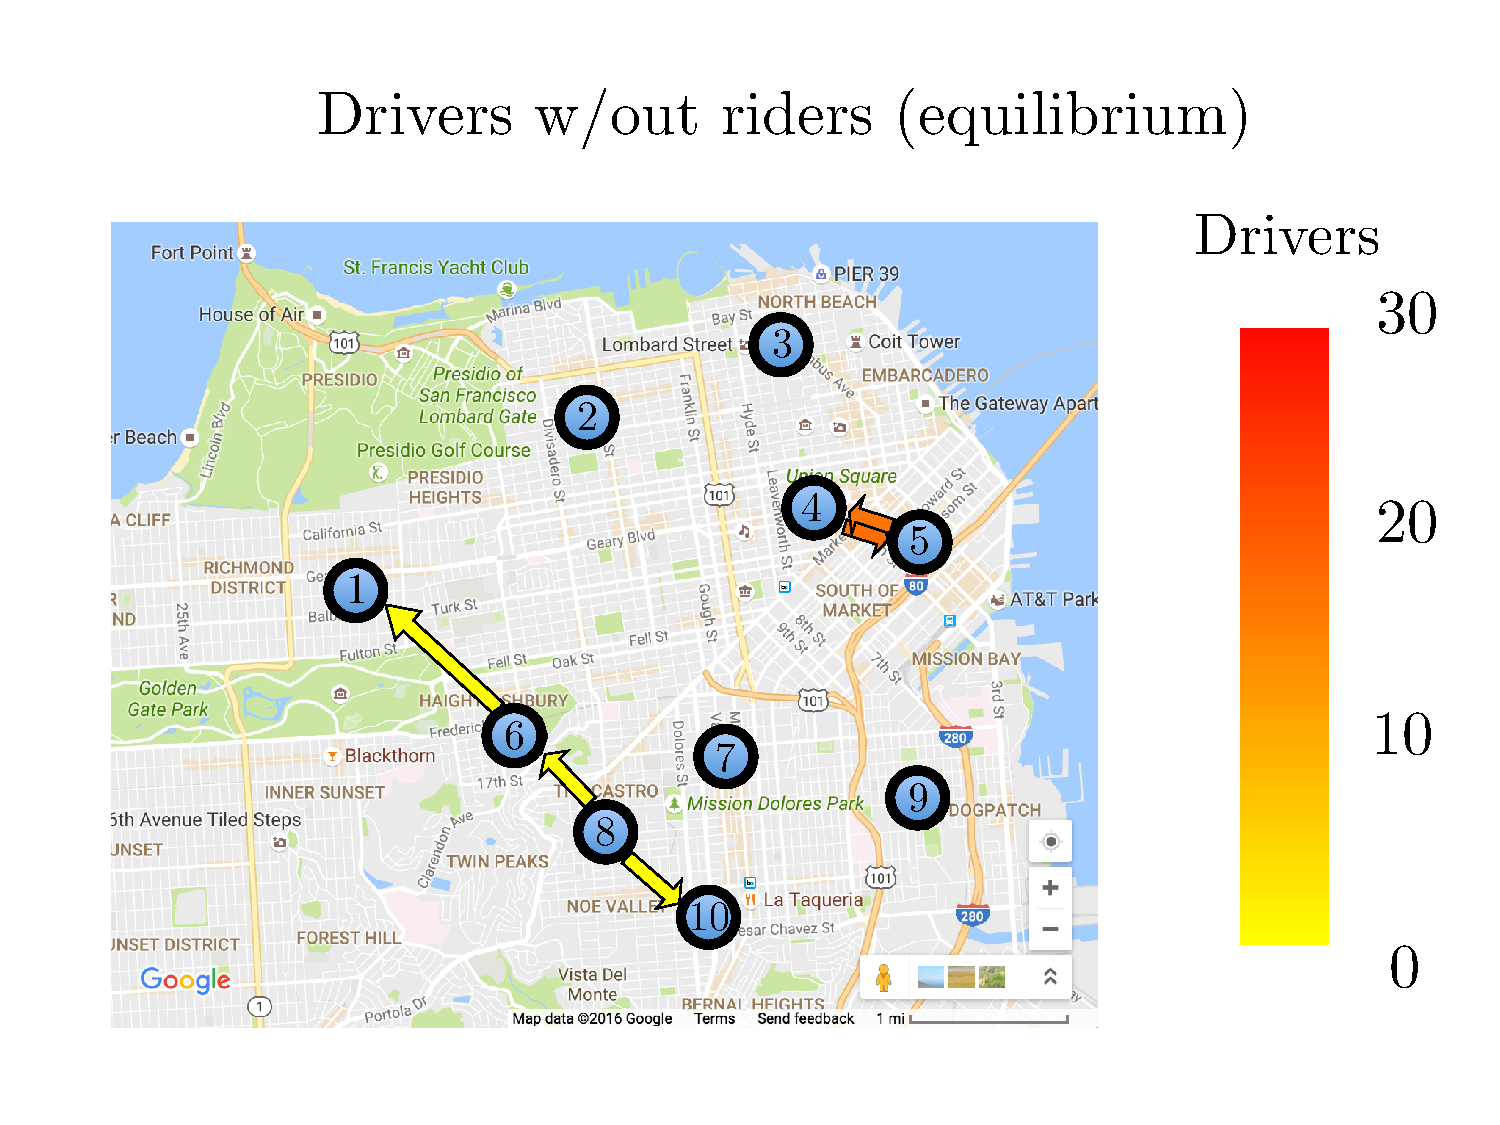
\includegraphics[width=0.25\textwidth]{figs/noriderseq.png}
%}
%\subfloat[\label{fig:noriderssoc}]{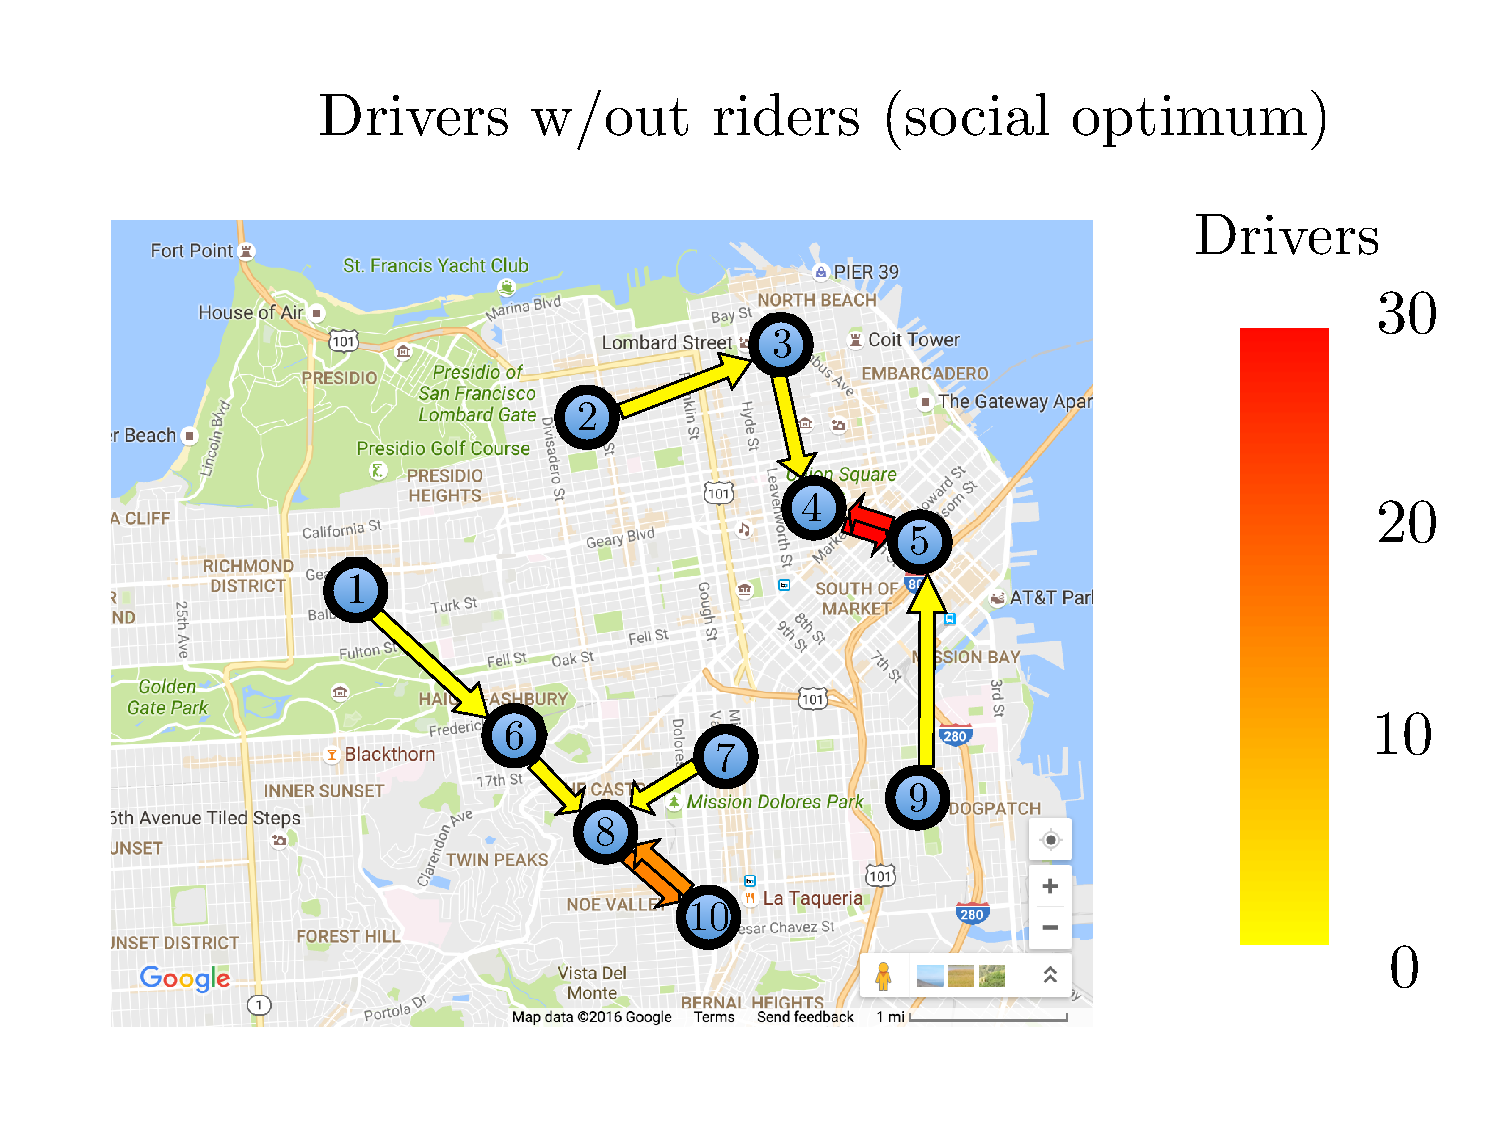
\includegraphics[width=0.25\textwidth]{figs/noriderssoc.png}
%}
\caption{Steady state distribution of drivers at each node under the (a) equilibrium strategies and (b) socially optimal strategies showing the portion of drivers that take riders and the portion that do not take riders.   
Drivers transitioning between nodes without riders in the (c) equilibrium case and (d) under the socially optimal strategies. }
\label{fig:nodesinf}
\end{figure}
\begin{figure}
\center
\subfloat[\label{fig:nodesinfeq}]{\includegraphics[width=0.5\textwidth]{figs/state7}
} 
\caption{Time profile of state 7 in unconstrained optimal solution and unconstrained optimal solution with exact penalty}
\label{fig:state7}
\end{figure}

% We compute both the equilibrium strategies and the socially optimal strategies in the infinite horizon game.  Figure \ref{fig:nodesinf} shows the steady state distribution of drivers at the nodes in both cases including the portion that take riders and the portion that do not as well as the transitions that drivers make without riders.  % without riders Figure \ref{fig:noriders} shows the the portion of the population that is making transitions without riders.  Interestingly, the socially optimal strategies involve more drivers making trips without riders.  
% \begin{figure}
% \center
% \subfloat[\label{fig:nodesinfeq}]{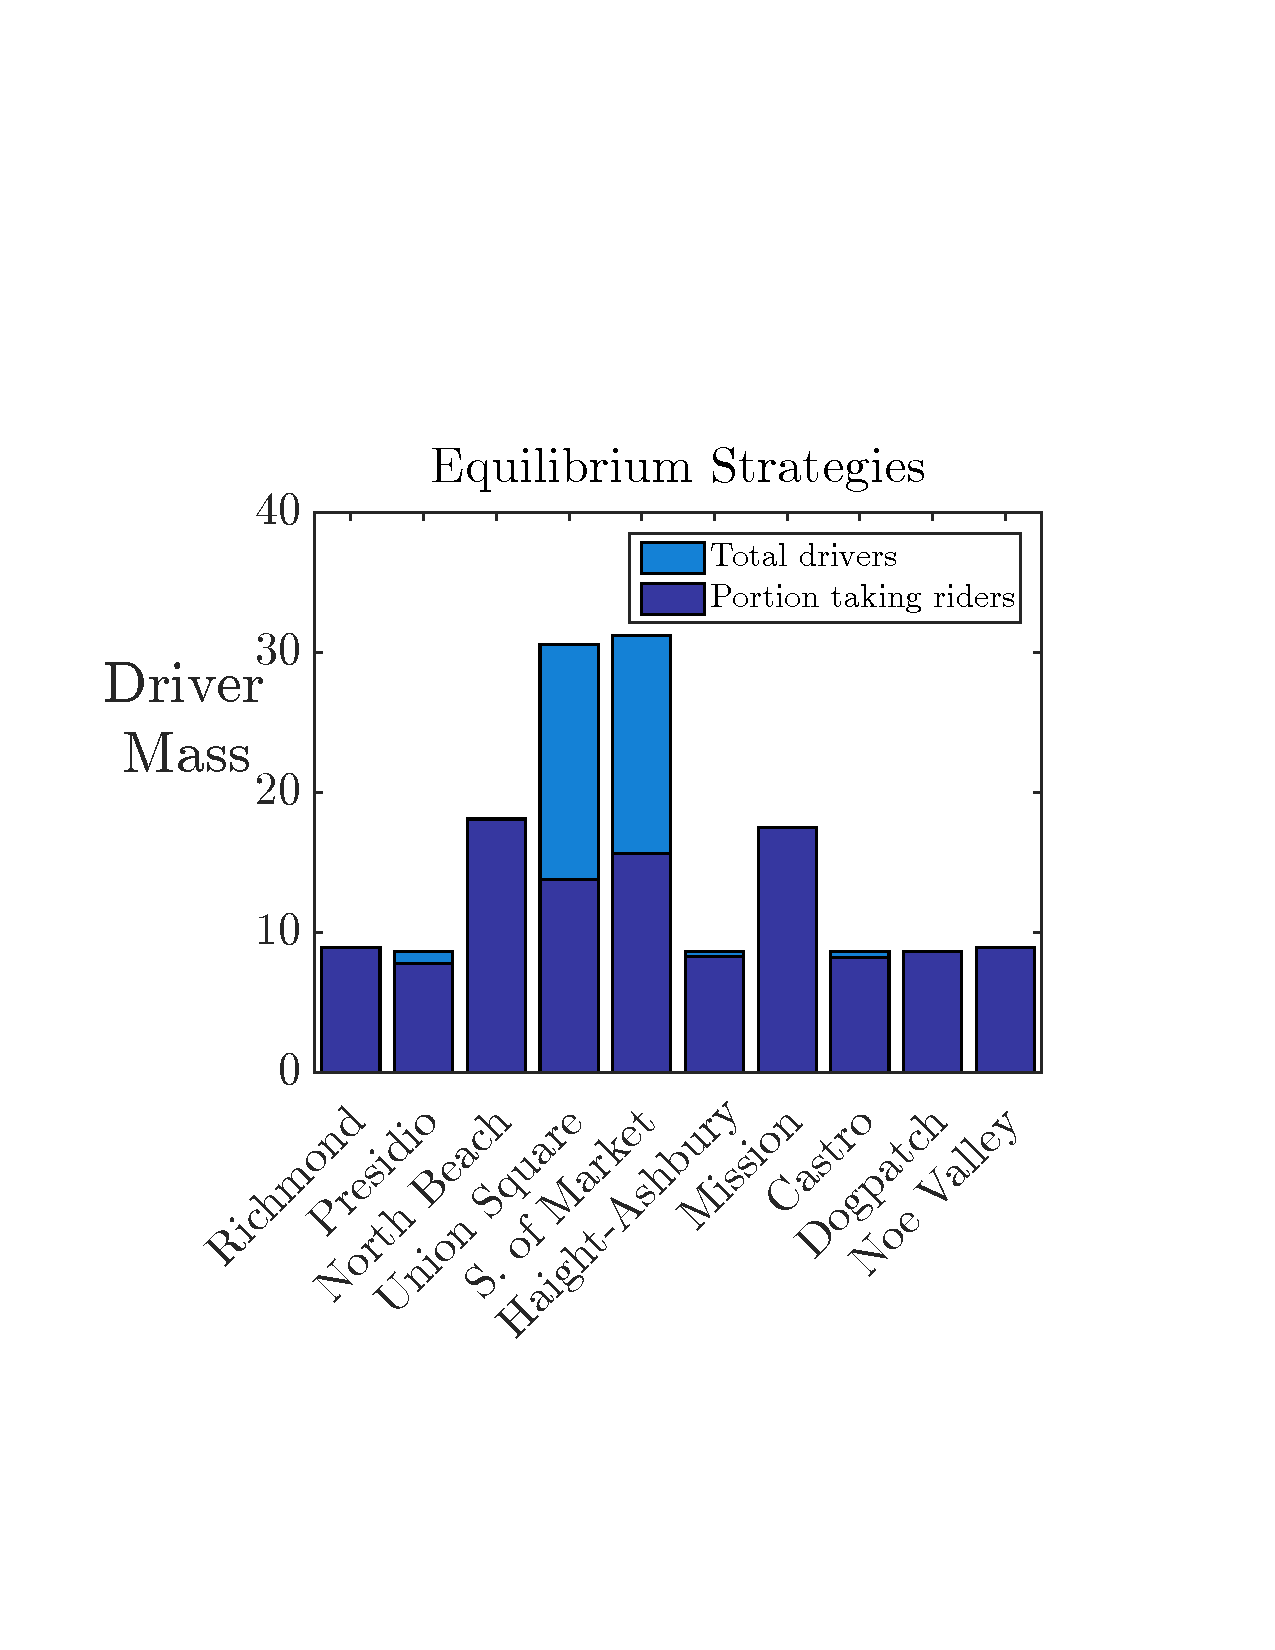
\includegraphics[width=0.23\textwidth]{figs/nodesinfeq.pdf}
% } 
% \subfloat[\label{fig:nodesinfsoc}]{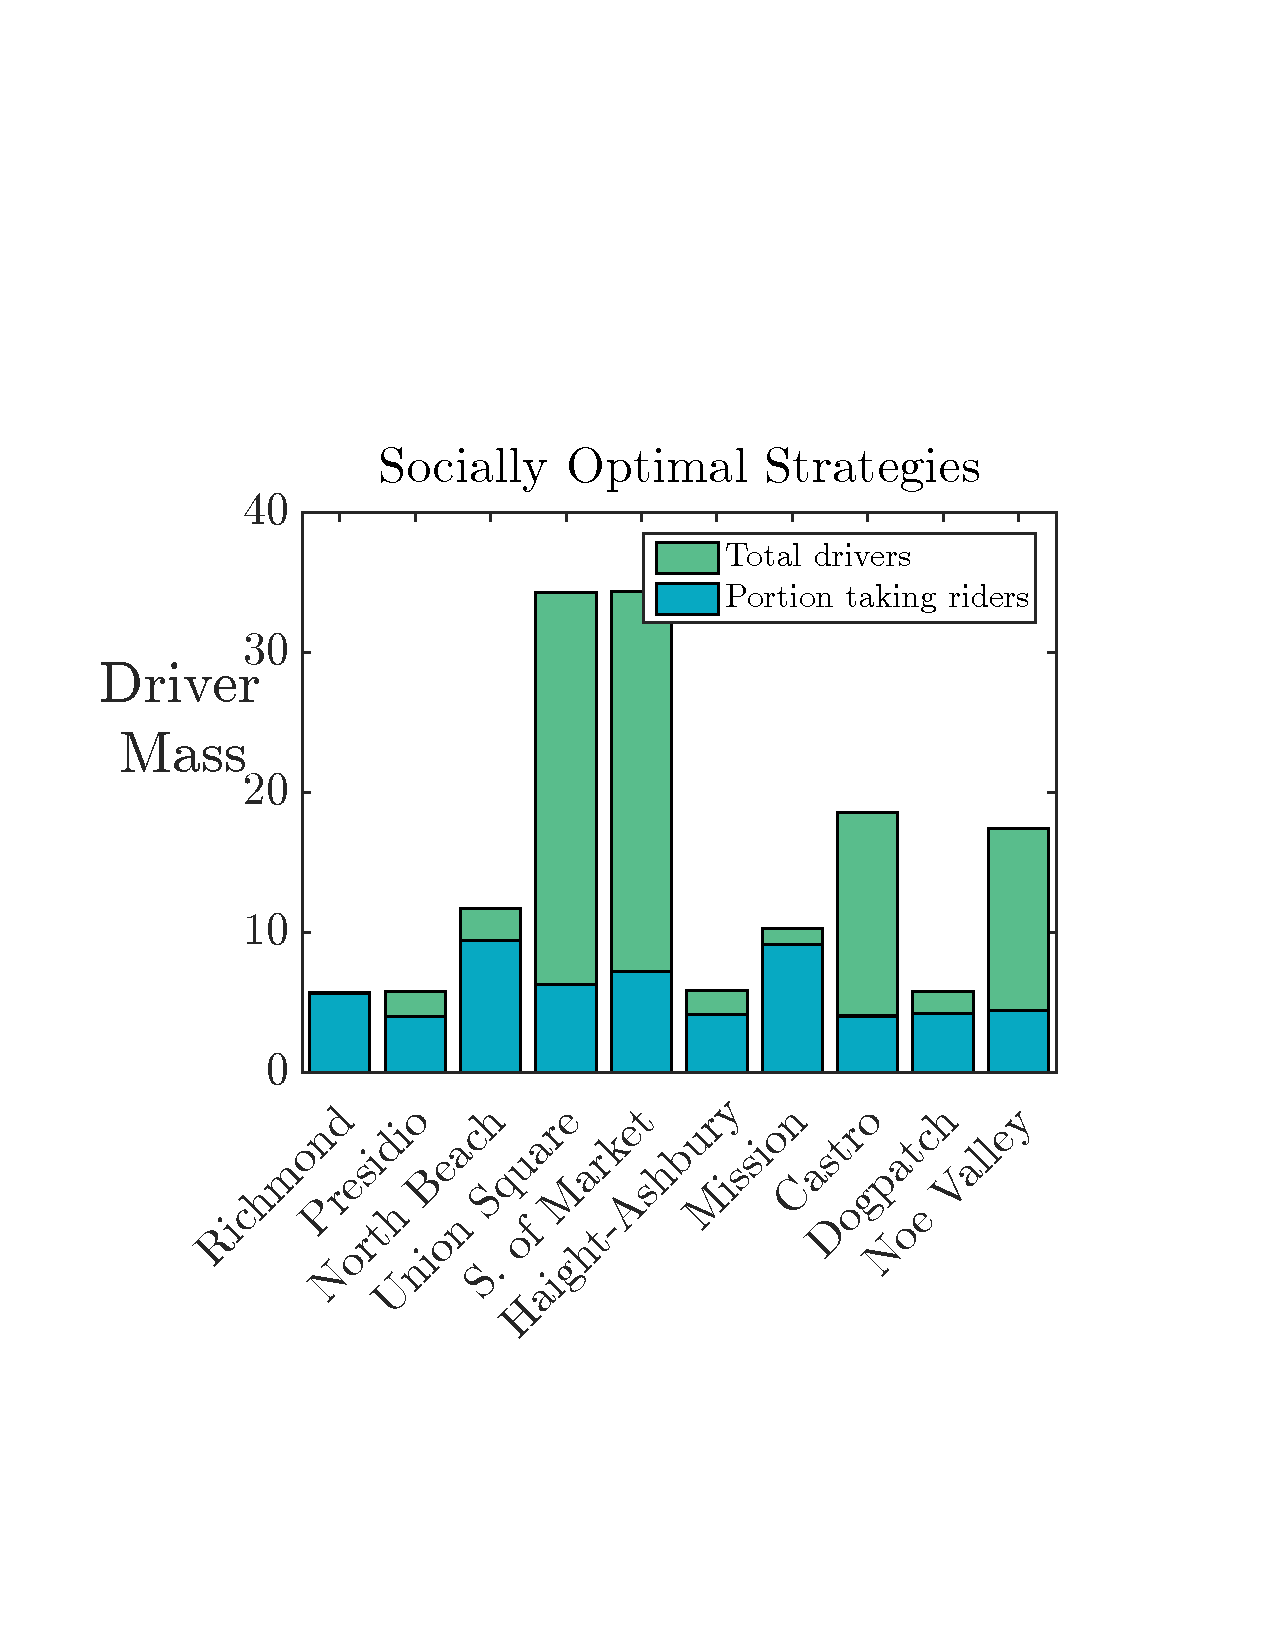
\includegraphics[width=0.23\textwidth]{figs/nodesinfsoc.pdf}
% }
% %\\
% %\subfloat[\label{fig:noriderseq}]{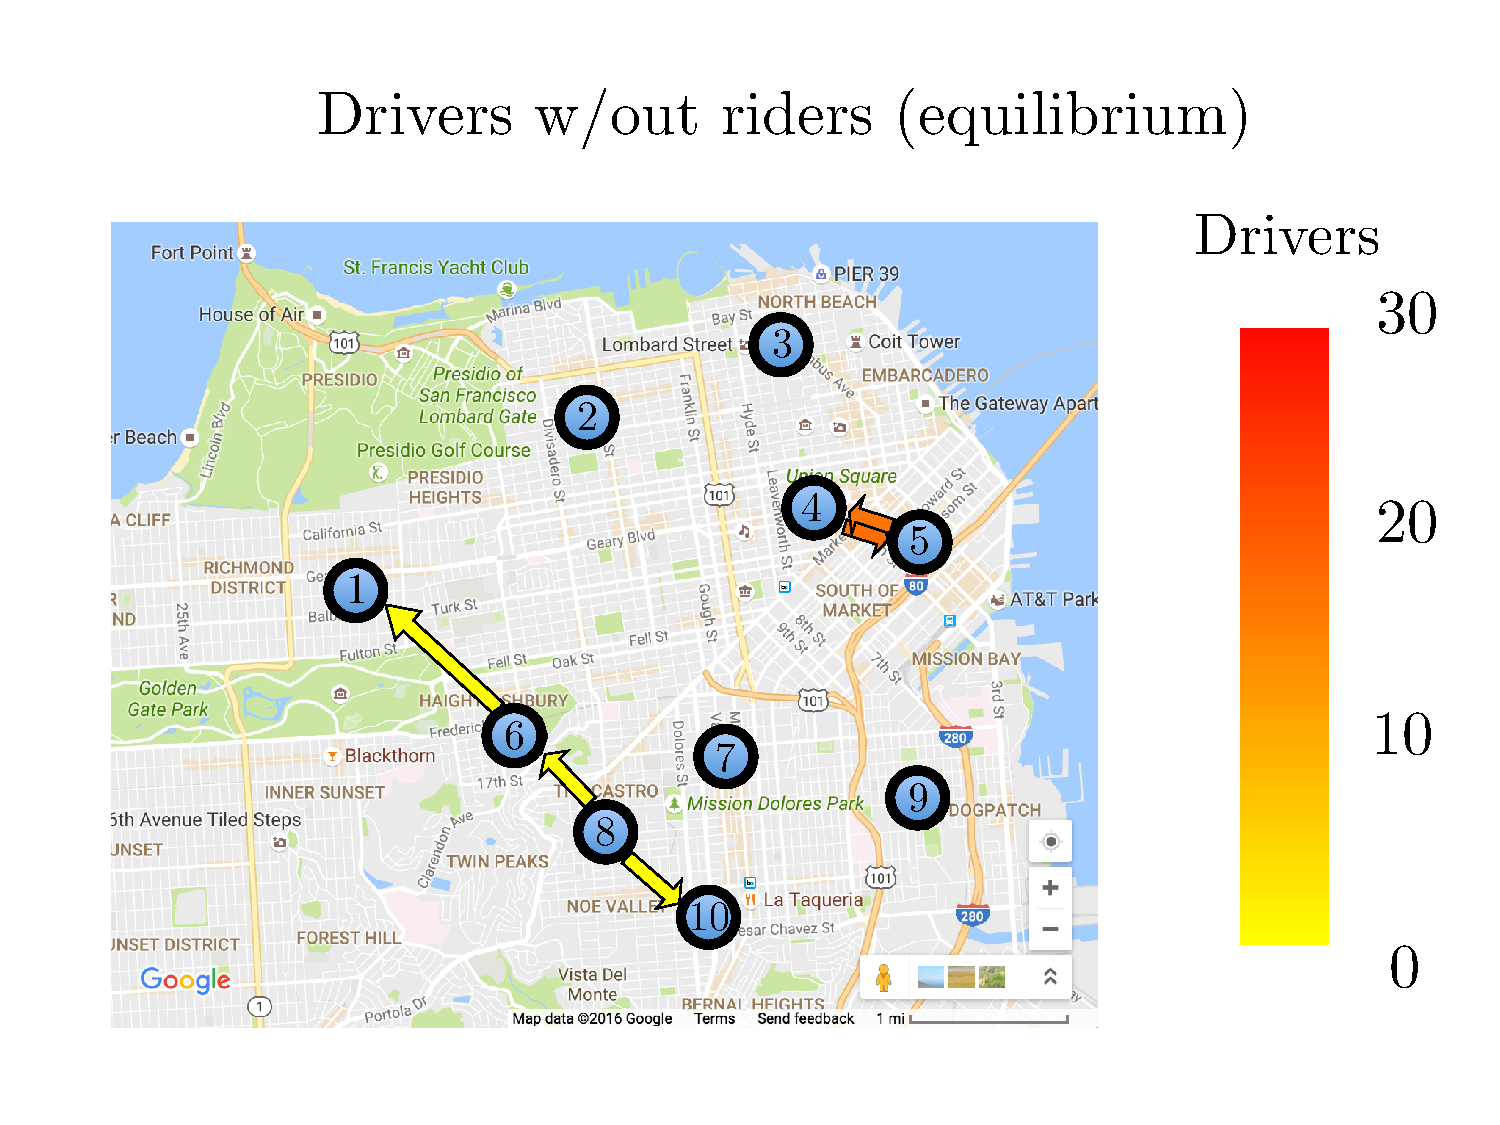
\includegraphics[width=0.25\textwidth]{figs/noriderseq.png}
% %}
% %\subfloat[\label{fig:noriderssoc}]{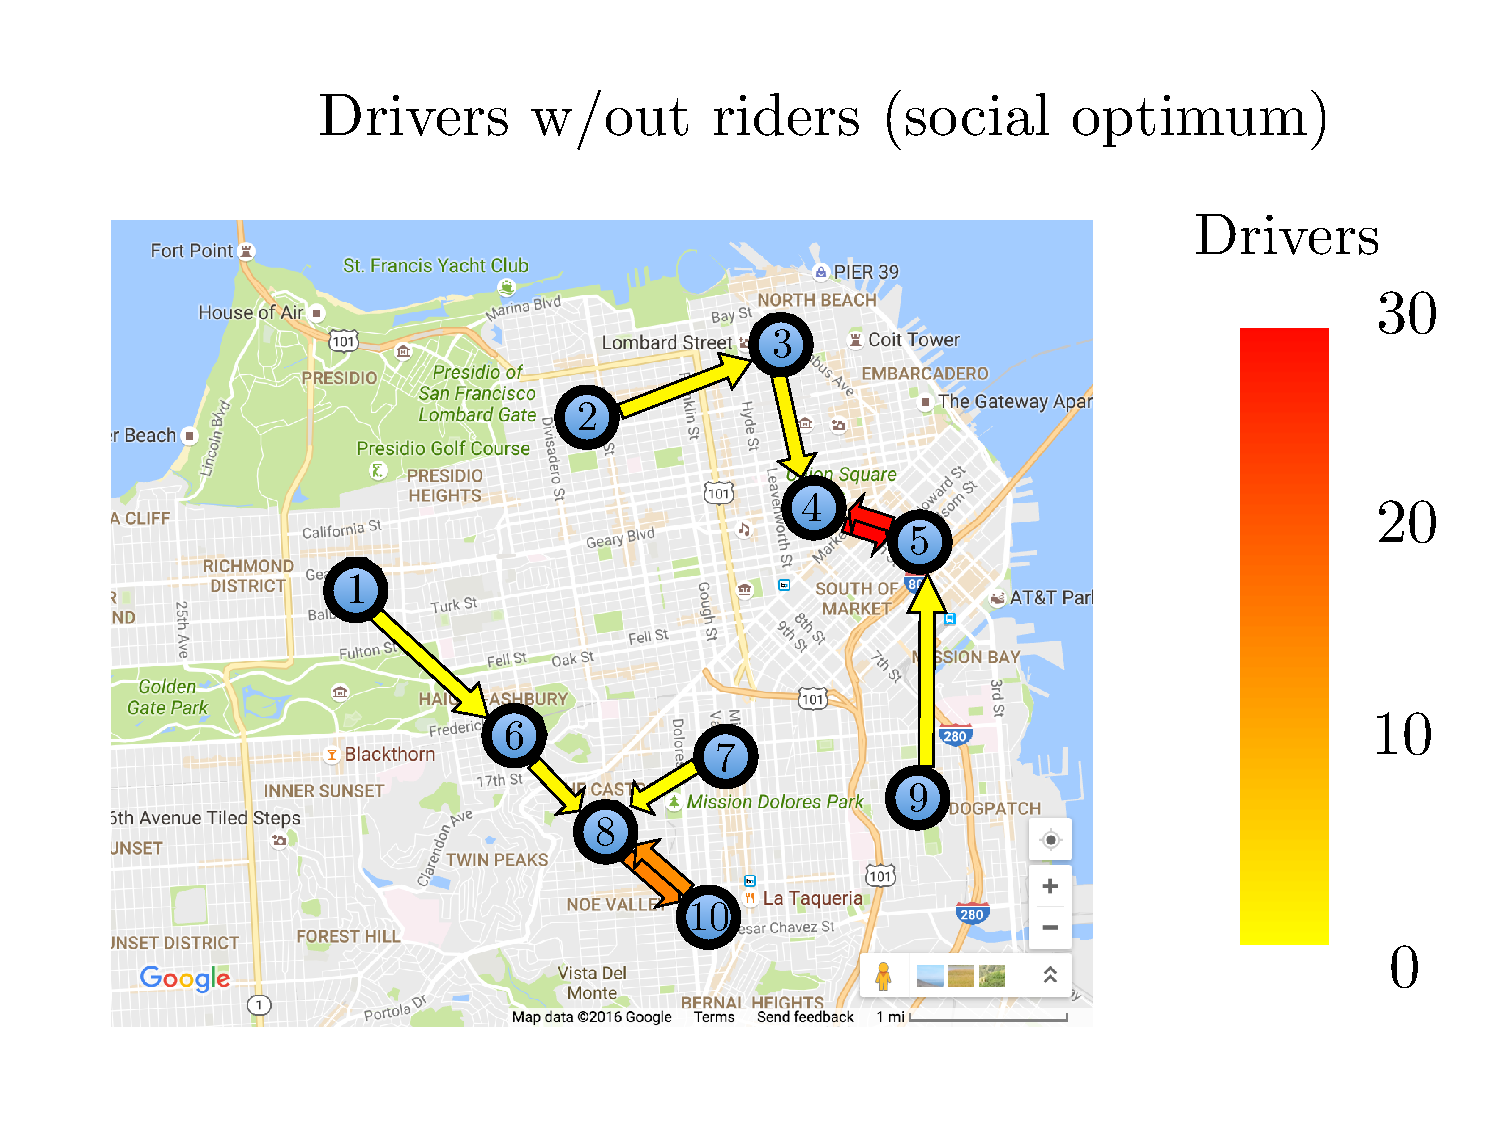
\includegraphics[width=0.25\textwidth]{figs/noriderssoc.png}
% %}
% \caption{Steady state distribution of drivers at each node under the (a) equilibrium strategies and (b) socially optimal strategies showing the portion of drivers that take riders and the portion that do not take riders.   
% Drivers transitioning between nodes without riders in the (c) equilibrium case and (d) under the socially optimal strategies. }
% \label{fig:nodesinf}
% \end{figure}



% \subsection{Circling for parking}
% \label{sec:circling}

% Another application of this model is determining the optimal strategies for urban drivers looking for places to park.  A sample set of city blocks shown in Figure \ref{fig:dualnums}.  We solve the problem on the dual graph as it allows us more freedom to restrict certain transitions (left turns, U-turns, etc.).  The actions associated with each state are either park, $a_p$, or make one one of the allowed turns stipulated in the following table (dependent on the intersection).
% \begin{center}
% \begin{tabular}{|c|cccc|}
% \hline
% Park & Straight & L-turn & R-turn & U-turn \\
% \hline
% $a_p$ & $a_s$ & $a_l$ & $a_r$ & $a_u$ \\
% \hline
% \end{tabular}
% \end{center}



% % of the allowed turn  actionsWe write down a reward function for each node (block face) that represents the expected waiting time to find an open space.  %The loss for transitioning from block face $j$ to block face $i$ is the loss experienced on block face $i$.  
% %Figure \ref{fig:dualgraph} shows the graph abstraction of several block faces.  We treat streets as nodes rather than intersection since it allows greater control over which turns drivers are allowed to make.  




% %
% %
% %\begin{figure}
% %\begin{center}
% %\includegraphics[scale=0.4]{mdp/figs/dualnums.png}
% %\caption{Block faces and allowed transitions.}
% %\label{fig:dualnums}
% %\end{center}
% %\end{figure}
% %

% The expected waiting time for a given member of the population is related to the rate at which spots become available and the probability that a driver will park given there is a parking spot open.  This last component depends on the number of other drivers on the block face.  For the probability of finding an empty spot, we draw inspiration from a queuing model where customers are selected randomly from a queue.  Each block face $s$ has $c_s$ spots and each spot becomes available at a rate of $\gamma_s$ (in units of car/min).  The total cost of driving by each block face is given by
% \begin{align}
% R_t[s,\ell_j(x) & = M_{j} p_j + \Big((C_j)_\text{wait}+M_j \Big) (1 - p_j)
% %R_{ij}(x) & = - (C_{ij})_{\text{trans}} - M_{i} p_i - (C_i)_\text{wait} (1 - p_i)
% \end{align}
% %Here $(C_{ij})_{\text{trans}}$ depends on the characteristics of the intersection, whether the transition is a right or left turn, whether it is a stop sign or traffic light, etc.  
% Here, $M_j$ is the cost of parking and $(C_j)_\text{wait}$ is the cost of waiting for a space which we take to be the $(C_j)_\text{wait} = \tau\Delta t_j$ where $\tau$ is a time vs. money tradeoff parameter and $\Delta t_j$ is the average amount of time spent on block face $j$.  The 
% probability of an individual driver getting a parking spot, $p_j$, is given by
% \begin{align}
% p_j & = \Big(1-e^{-c_j\gamma_j \Delta t_j}\Big) \frac{1}{1+x_j} %\sum_j x_{ij}} 
% \end{align}
% This equation consists of two parts.  The first is the probability that a space opens up in the time the driver spends on the block face.  The second part is the probability that an individual driver of the population on the edge gets that space.  This second term is 1 when there is 0 mass on the edge, $\frac{1}{2}$ when there is a mass of 1 other driver on the edge, $\frac{1}{3}$ when there is a mass of 2 other drivers on the edge, etc.  

% The full loss function can be rewritten as
% \begin{align}
% \ell_j(x) = 
% %l_{ij}(x)  = l_i(x) = 
% \underbrace{
% \Big(M_j + (C_j)_\text{wait}\Big)
% }_{a_j} 
% \underbrace{-
% (C_j)_\text{wait}\Big(1-e^{-c_j\gamma_j \Delta t_j}\Big)
% }_{b_j}
% \frac{1}{1+ x_j} %\sum_j x_{ij}}
% %R_{ij}(x)  = - (C_{ij})_{\text{trans}} - (C_i)_\text{wait}  + \Bigg((C_i)_\text{wait}-M_{i}\Bigg)\frac{1-e^{-c_i\mu_i \Delta t_i}}{\sum_j x_{ij}}
% \end{align}
% %We note that it is important for $M_i > (C_i)_\text{wait}$, otherwise no one would want to park.  
% The potential function is then given by
% \begin{align}
% %F(x) & = \sum_j \int_0^{\sum_j x_{ij}} l_i(u) \ du \\
% %F(x) & = \sum_j \left[ a_i \sum_j x_{ij} + b_i \ln\left(1+\sum_j x_{ij} \right)\right]
% F(x) = \sum_j \int_0^{x_j} \ell_j(u) \ du 
% = \sum_j \bigg[ a_j x_j + b_i \ln\big(1+x_j \big)\bigg]
% \end{align}
% We use the following parameter values (Table. \ref{commonParamVal}) for all streets, while the number of parking spaces are given by Table. \ref{spaceParam}.
% \begin{center}\label{commonParamVal}
% \begin{tabular}{|cccc|}
% \hline
% $\Delta t_j $ (min)  & $\gamma_j$ (1/hr) & $M_j$ (\$) & $\tau$ ($\$$/min) \\
% \hline
% 0.5 &  1/120 &  5 & 0.5\\
% \hline
% \end{tabular}
% \end{center}


% \begin{center}\label{spaceParam}
% \begin{tabular}{|c|ccccccc|}
% \hline
% Street & 
% 1-6 & 7-8 & 9-10 & 11-14 & 15-16 & 17-18 & 19 -24 \\
% \hline
% Num. spaces $(c_j)$ &
% 20 & 10 & 20 & 10 & 20 & 10 & 20 \\
% \hline
% \end{tabular}
% \end{center}
% The streets are numbered in Figure \ref{fig:dualnums}.  

% % We consider this game in the infinite horizon case with deterministic transitions.  In Figure \ref{fig:circles}, we look at the traffic distribution at the Wardrop equilibrium, at the social optimum, and when the population members use a uniform turning strategy.  We note that one application of this model could be determining how to vary parking prices between streets in order to improve congestion since even in this simple scenario the Nash solution is suboptimal.  We also note that a model like this could be integrated with the queue-routing game developed in Chapter \ref{chap:park} to provide a more sophisticated model of parking behavior.  

% \begin{figure*}
% \center
% \subfloat[\label{fig:dualnums}]{\includegraphics[width=0.45\textwidth]{figs/dualnums.pdf}}
% \hspace{0.1in}
% \subfloat[\label{fig:circlenash}]{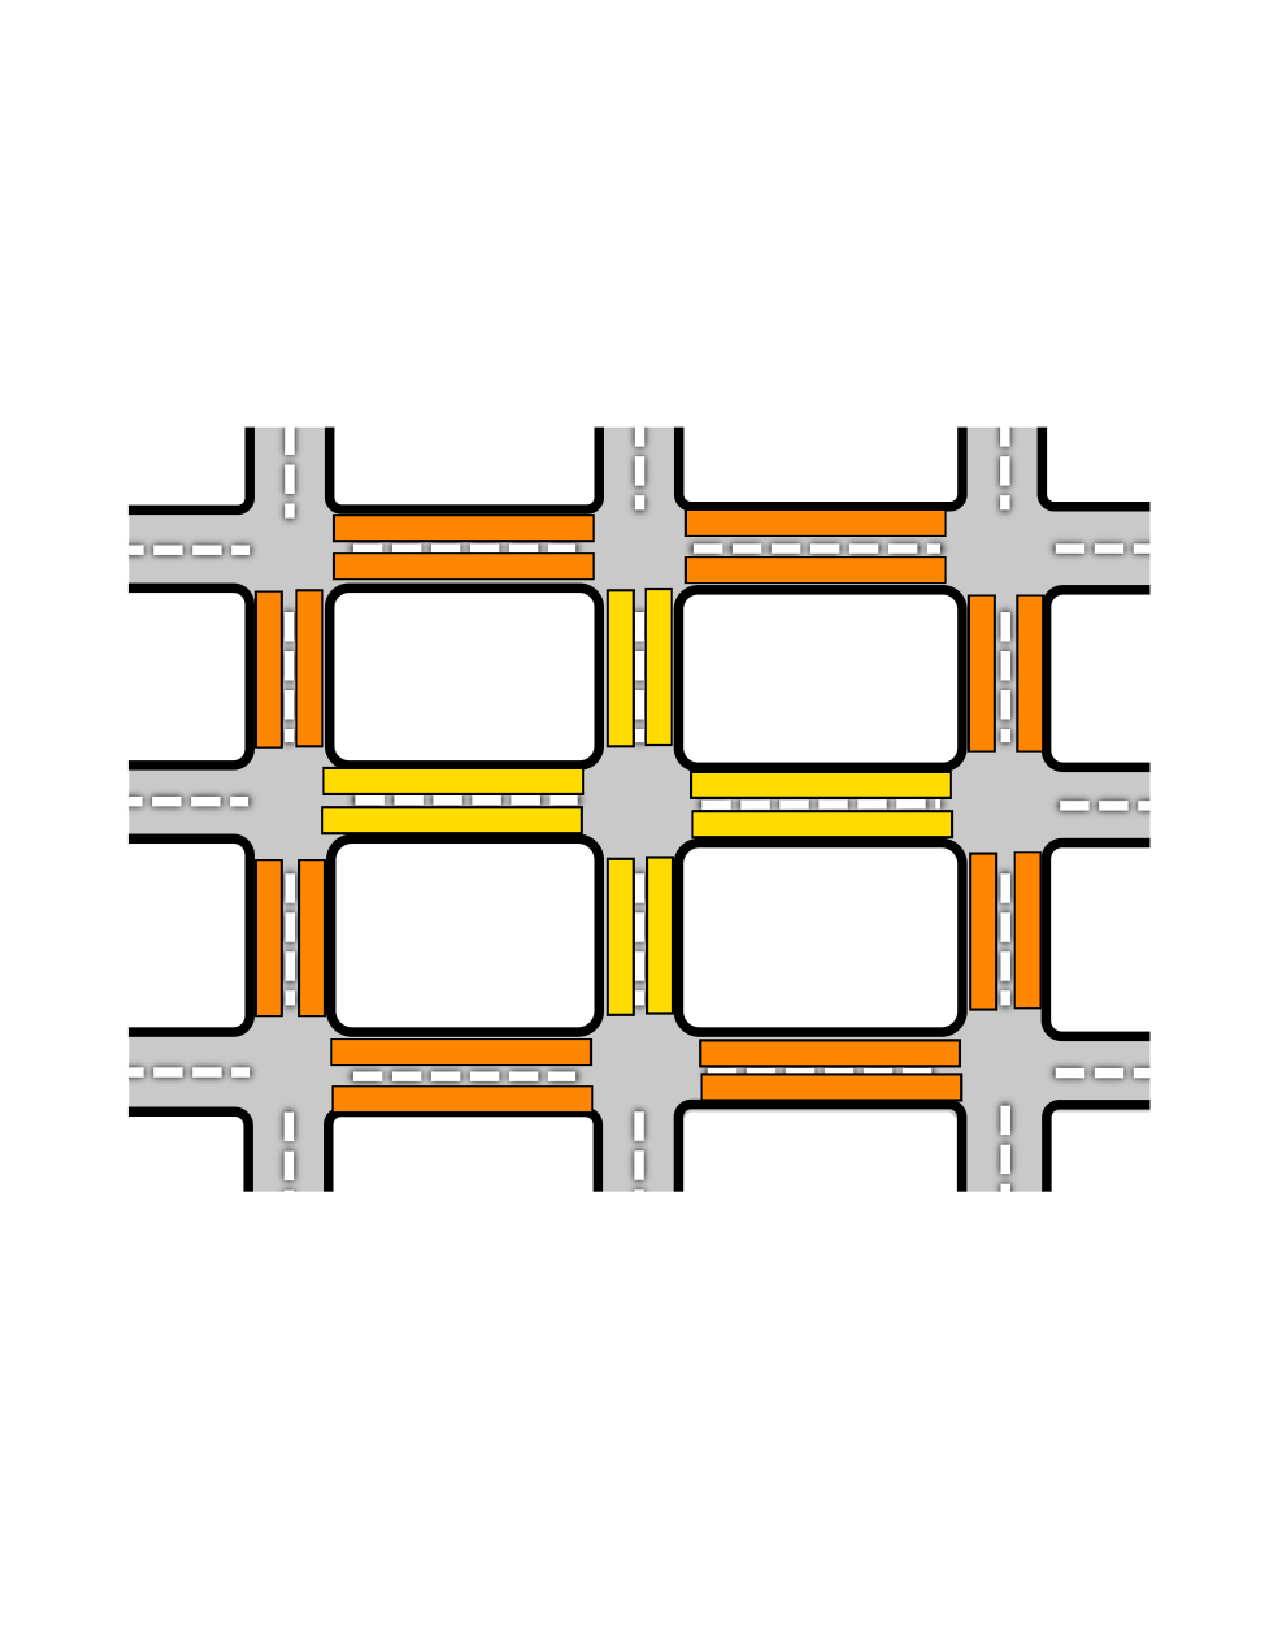
\includegraphics[width=0.45\textwidth]{figs/circle_nash.pdf}}
% \\
% \subfloat[\label{fig:circlesoc}]{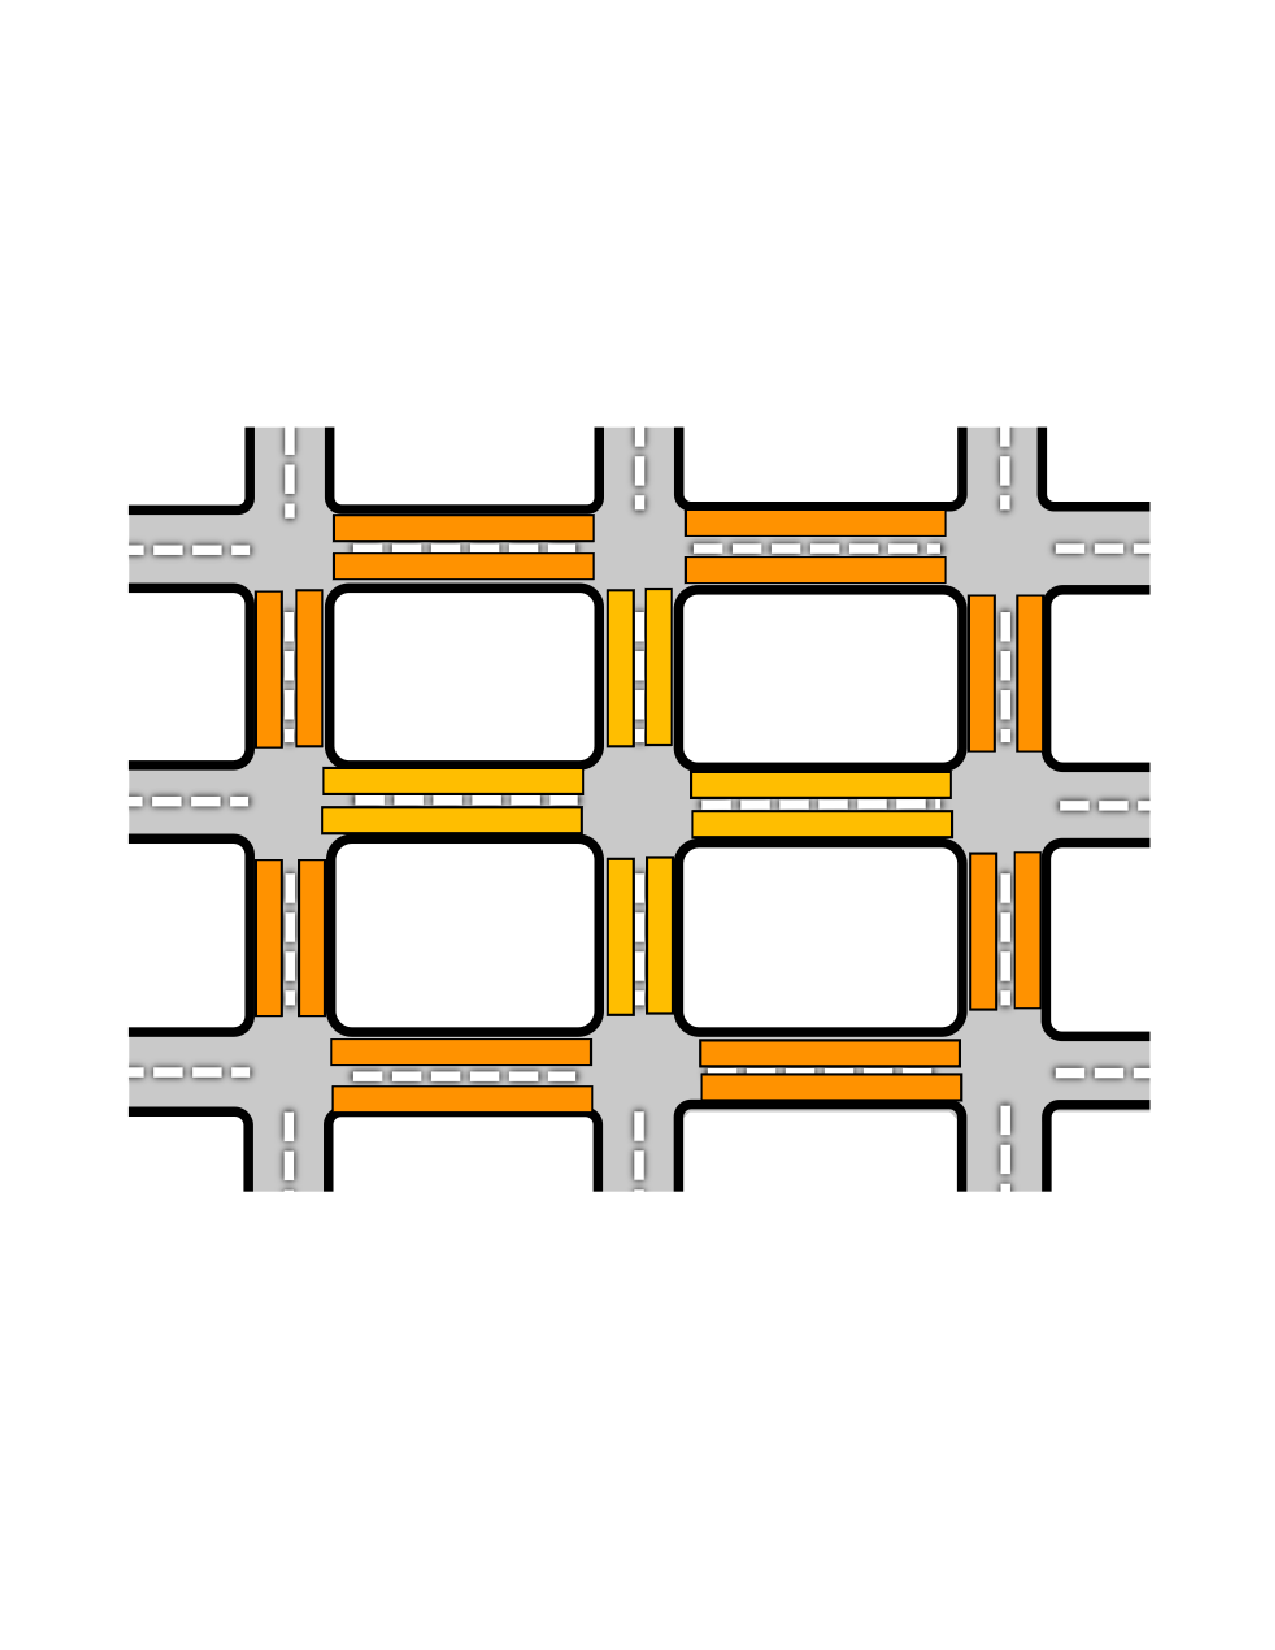
\includegraphics[width=0.45\textwidth]{figs/circle_soc.pdf}}
% \hspace{0.1in}
% \subfloat[\label{fig:circleunif}]{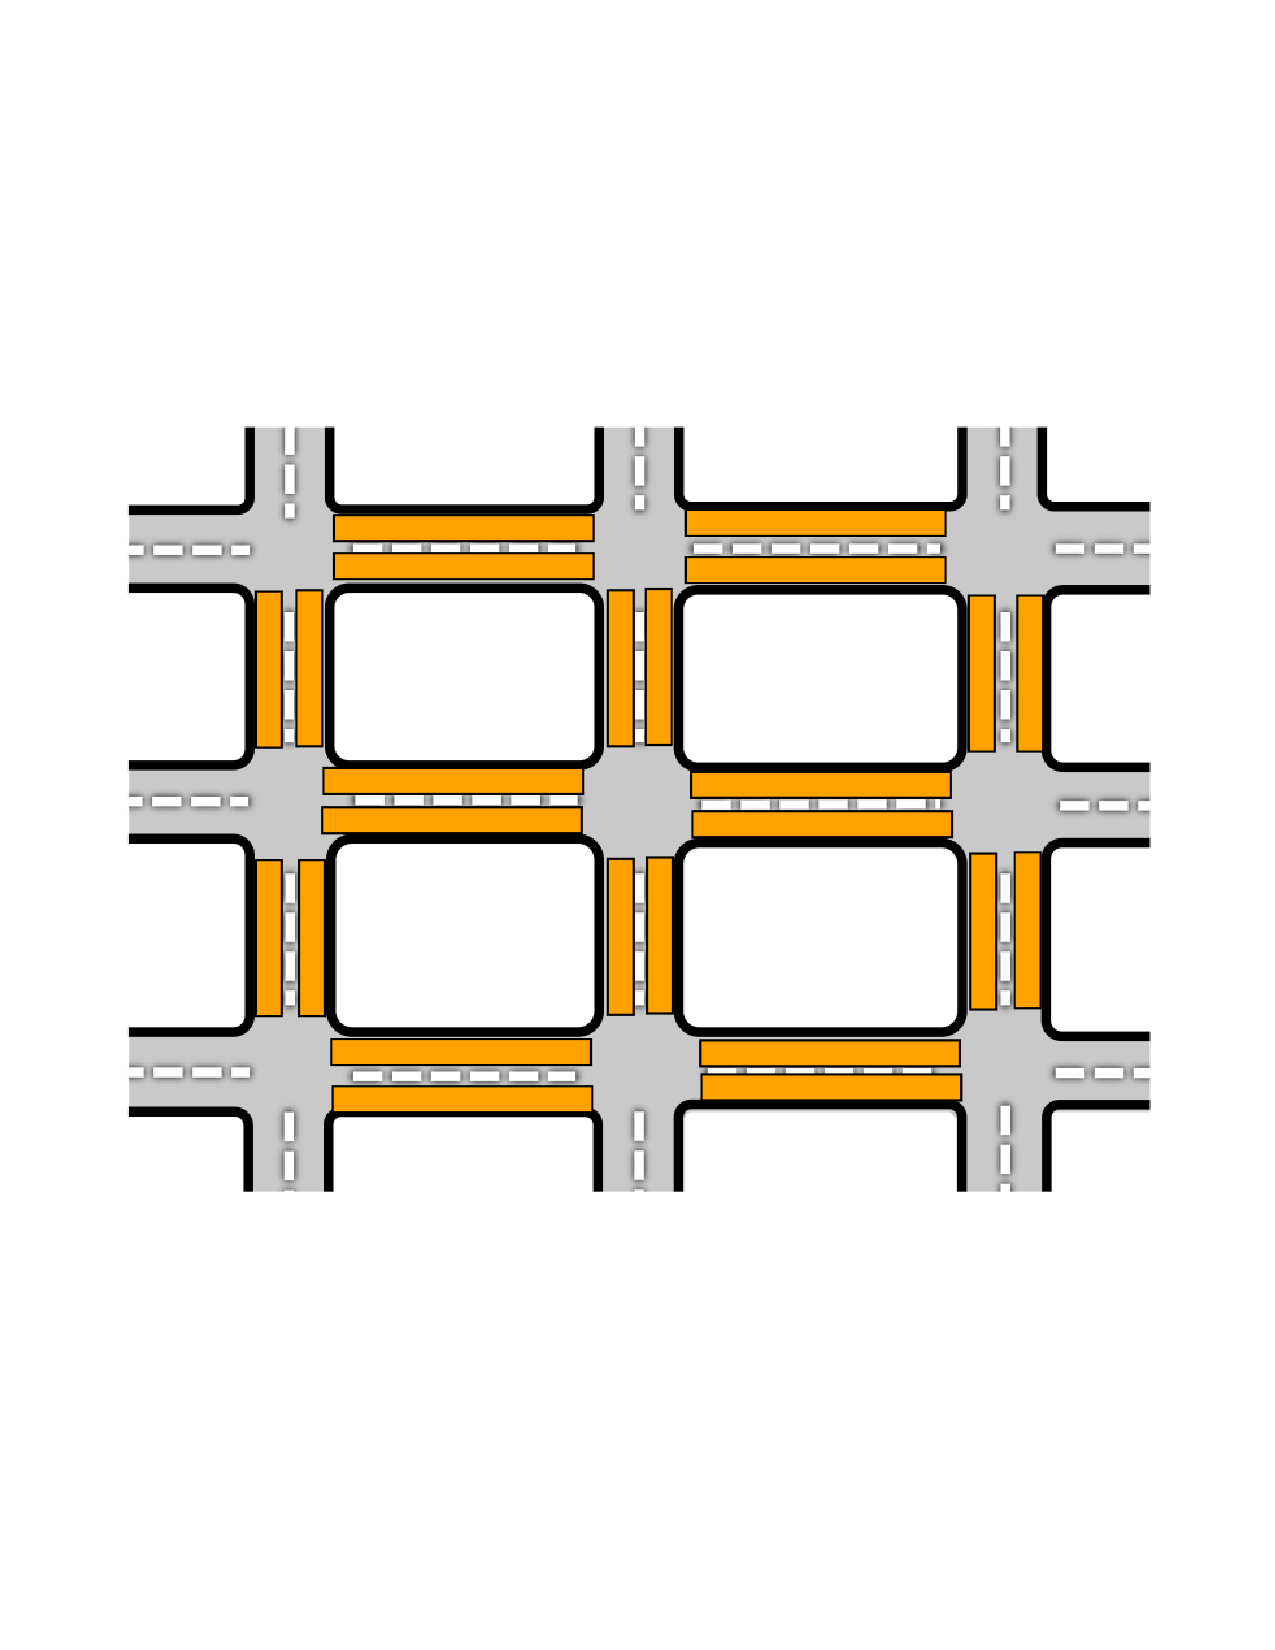
\includegraphics[width=0.45\textwidth]{figs/circle_unif.pdf}}
% \hspace{0.1in}
% \subfloat[]{\includegraphics[width=0.05\textwidth]{figs/circle_scale.png}}
% \caption{(a) Block faces and allowed transitions. (b) Wardrop equilibrium.  (c) Social optimum.  (d) Uniform turns.  (e) Scale (cars).}
% \label{fig:circles}
% %    \label{fig:amgrids}
%  \end{figure*}




\section{Conclusions}\label{conclusion}


\bibliographystyle{IEEEtran}
\bibliography{reference}

\end{document}